\documentclass[tikz,border=5pt]{standalone}
\usepackage[utf8]{inputenc}
\usepackage[T1]{fontenc}
\usepackage{lmodern,amsmath,amssymb}
\usepackage[american]{circuitikz}
\usepackage{pgfplots}
\pgfplotsset{compat=1.18}
\usetikzlibrary{circuits.logic.US,positioning,calc,arrows.meta,patterns,shapes.geometric}
\definecolor{Primary}{HTML}{1F77B4}
\begin{document}
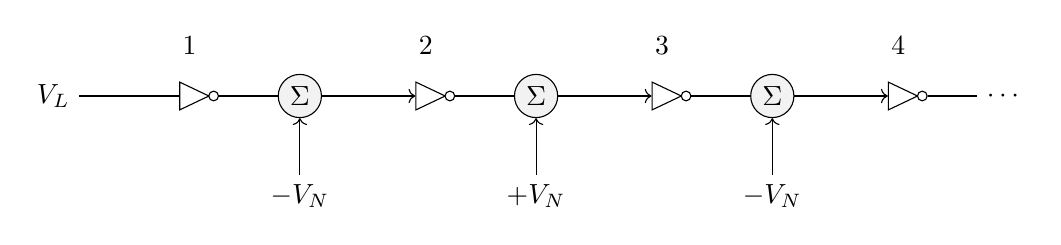
\begin{tikzpicture}[circuit logic US,every circuit symbol/.style={minimum size=9mm}]\node[not gate US,draw] (g0) at (0,0){};\node[above] at (0,.4){1};\node[not gate US,draw] (g1) at (3,0){};\node[above] at (3,.4){2};\node[not gate US,draw] (g2) at (6,0){};\node[above] at (6,.4){3};\node[not gate US,draw] (g3) at (9,0){};\node[above] at (9,.4){4};\node[circle,draw,fill=gray!10,inner sep=2pt](s0)at(1.4,0){$\Sigma$};\draw(g0.output)--(s0.west);\draw[->](s0.east)--(g1.input);\draw[->](1.4,-1)node[below]{$-V_N$}--(s0.south);\node[circle,draw,fill=gray!10,inner sep=2pt](s1)at(4.4,0){$\Sigma$};\draw(g1.output)--(s1.west);\draw[->](s1.east)--(g2.input);\draw[->](4.4,-1)node[below]{$+V_N$}--(s1.south);\node[circle,draw,fill=gray!10,inner sep=2pt](s2)at(7.4,0){$\Sigma$};\draw(g2.output)--(s2.west);\draw[->](s2.east)--(g3.input);\draw[->](7.4,-1)node[below]{$-V_N$}--(s2.south);\draw(-1.4,0)node[left]{$V_L$}--(g0.input);\draw(g3.output)--(10,0)node[right]{$\cdots$};\end{tikzpicture}
\end{document}
